\subsection{Free Damped Vibrations ($b > 0$)}
We need to consider three cases where the discriminant $\Delta = b^2 - 4mk$ is positive, zero, and negative. 

\subsubsection{Overdamped ($\Delta > 0$)}
This is the simplest and easiest case to deal with because our two roots, $r_1$ and $r_2$, are real and distinct. So, out solution is
\begin{equation*}
	y = C_1e^{r_1 t} + C_2e^{r_2 t}.
\end{equation*}
\begin{center}
	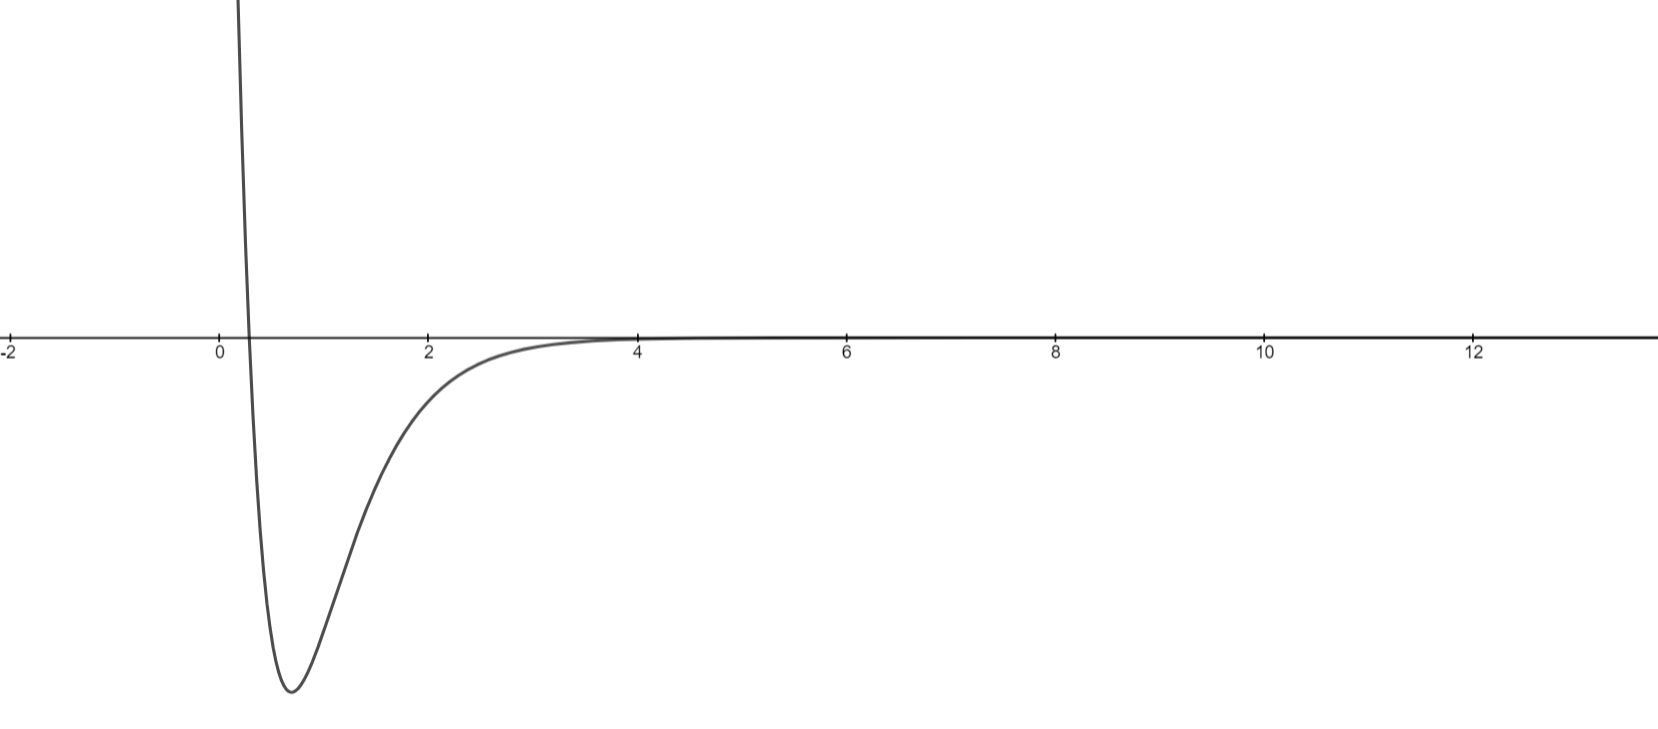
\includegraphics[width=0.5\textwidth]{./higherOrder/freeVibrs/overdamped.png}
\end{center}
We know that $r_1, r_2 < 0$, so
\begin{equation*}
	\lim\limits_{t \to 0}{C_1e^{r_1 t} + C_2e^{r_2 t}} = 0
\end{equation*}
meaning the mass's oscillation decays over time.
\subsubsection{Critically Damped ($\Delta = 0$)}
This case isn't much more difficult. The only difference is that because both roots $r_1$ and $r_2$ are $\frac{-b}{2m}$, we need an extra $t$ term in the solution. So, out solution is
\begin{equation*}
	y = C_1e^{r_1 t} + C_2te^{r_2 t}
\end{equation*}
\begin{center}
	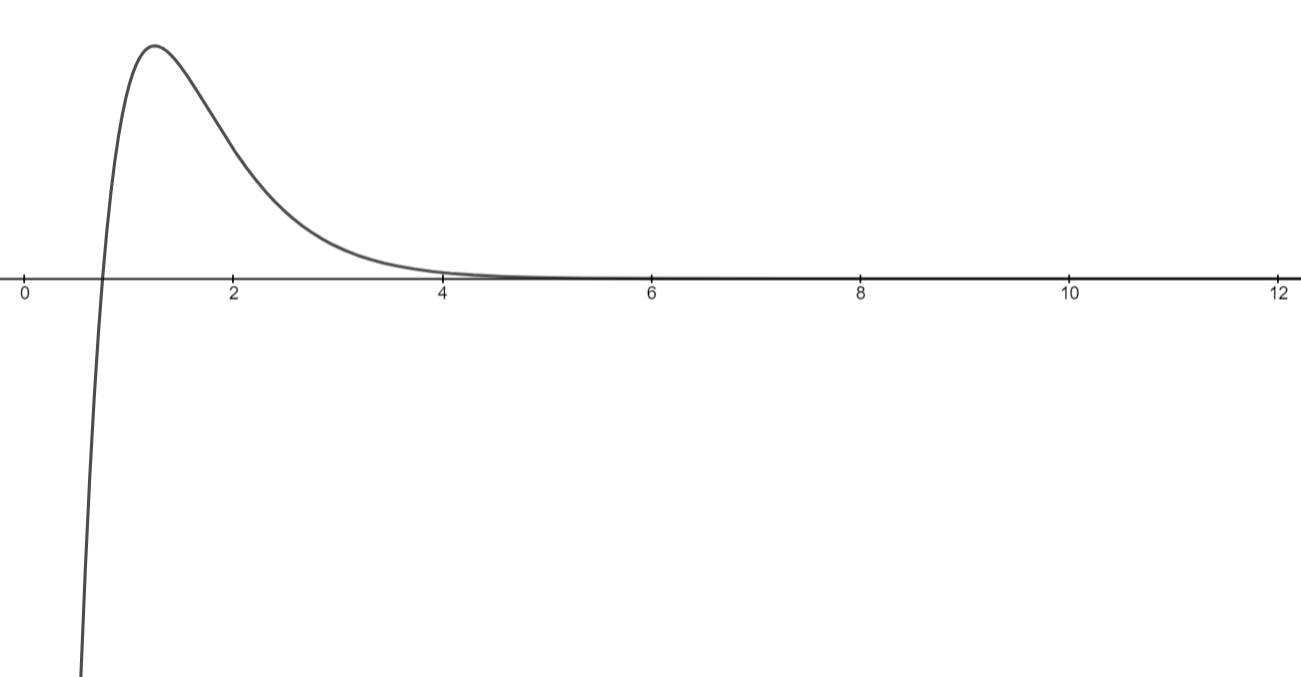
\includegraphics[width=0.5\textwidth]{./higherOrder/freeVibrs/criticallydamped.png}
\end{center}
Since both roots are once again negative,
\begin{equation*}
\lim\limits_{t \to 0}{C_1e^{r_1 t} + C_2te^{r_2 t}} = 0
\end{equation*}
meaning the mass's oscillation decays over time.
\subsubsection{Underdamped ($\Delta < 0$)}
This is probably the most complicated case.
Here, both roots are complex.
Specifically,
\begin{equation*}
	r = \frac{-b}{2m} \pm i\frac{\sqrt{\abs{\Delta}}}{2m}.
\end{equation*}
Letting the coefficient of the imaginary part be $\omega$,
\begin{equation*}
	r = \frac{-b}{2m} \pm i\omega.
\end{equation*}
So, our solution becomes
\begin{equation*}
	y = e^{\frac{-b}{2m} t}\left(C_1\cos{(\omega t)} + C_2\sin{(\omega t)}\right).
\end{equation*}
Rewriting in terms of $\cos$ and a phase shift,
\begin{equation*}
	y = Ae^{\frac{-b}{2m} t}\cos{(\omega t - \phi)} \text{ where }
	A = \sqrt{A^2 + B^2} \text{, } \phi = \begin{cases}
		\arctan{\left(\frac{B}{A}\right)} + \pi & A \leq 0 \\
		\arctan{\left(\frac{B}{A}\right)} & A > 0
	\end{cases}.
\end{equation*}
\begin{center}
	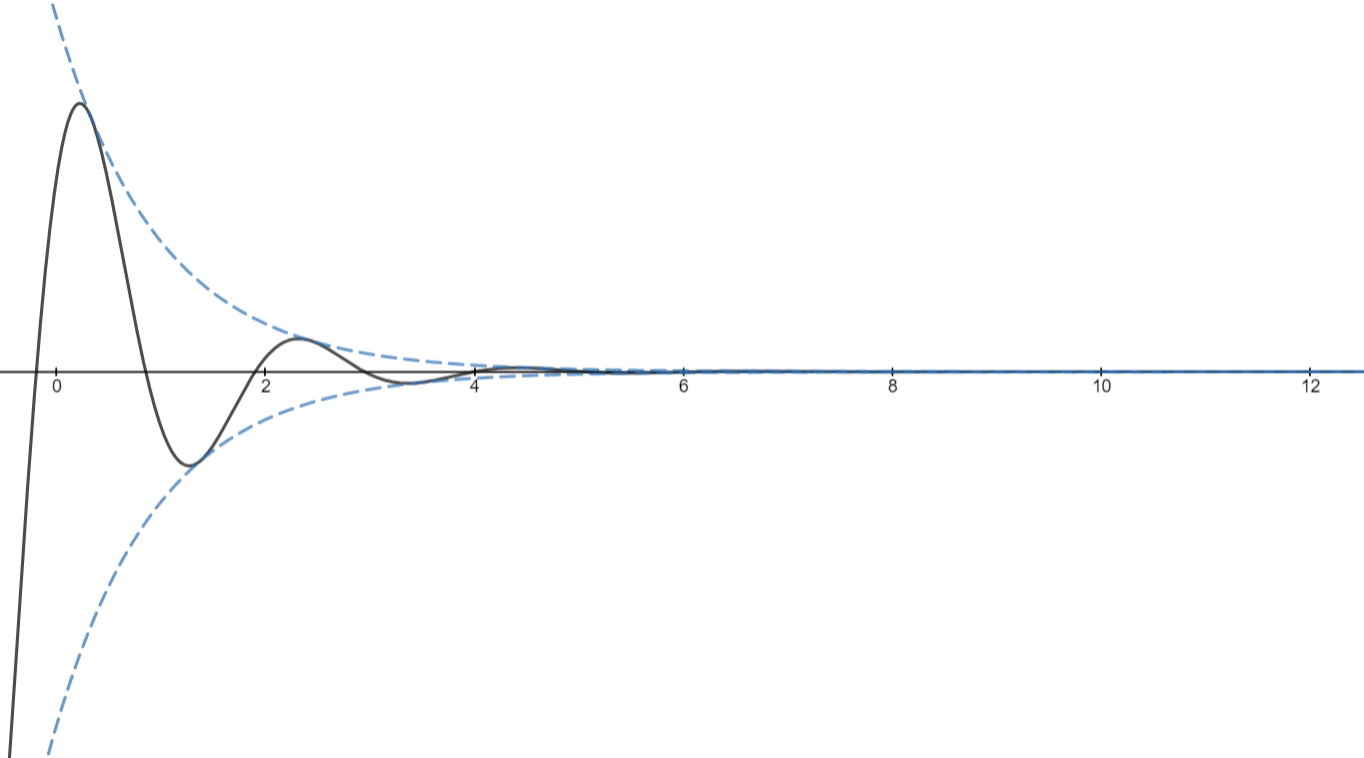
\includegraphics[width=0.5\textwidth]{./higherOrder/freeVibrs/underdamped.png}
\end{center}
Here, the exponential term dominates the limit, so
\begin{equation*}
	\lim\limits_{t \to 0}{Ae^{\frac{-b}{2m}t}\cos{(\omega t - \phi)}} = 0
\end{equation*}
meaning the mass's oscillation decays over time, bounded by the exponential curves. 

\begin{example}
	A 250g mass is attached to a spring with a constant of $k = 10\text{N/m}$. The mechanical impedance is 3$\text{kg}{s}$. Initially, the mass is at $y(0)=-1\text{m}$ and $y'(0)=2\text{m/s}$. Find an expression for $y(t)$, the position of the mass at time $t$. Write any oscillations as a $\cos$ and a phase shift. Is the system underdamped, critically damped, or overdamped?
\end{example}
\noindent
The IVP describing this scenario is
\begin{equation*}
	\begin{cases}
		\frac{1}{4}y'' + 3y' + 10y = 0 \\
		y(0) = -1 \\
		y'(0) = 2
	\end{cases}.
\end{equation*}
Solving the auxiliary equation,
\begin{equation*}
	\frac{1}{4}r^2 + 3r + 10 = 0 \implies r = \frac{-3 \pm \sqrt{3^2 - 4(1/4)(10)}}{2(1/4)} = -6 \pm 2i.
\end{equation*}
So, the general solution is
\begin{equation*}
	y = e^{-6t}\left(C_1\cos{(2t)} + C_2\sin{(2t)}\right).
\end{equation*}
Solving for $C_1$ and $C_2$,
\begin{equation*}
	y(0) = -1 = C_1 \implies C_1 = -1.
\end{equation*}
\begin{equation*}
	y' = e^{-6t}\left(-2C_1\sin{(2t)} + 2C_2\cos{(2t)}\right) + \left(C_1\cos{(2t)} + C_2\sin{(2t)}\right) \cdot -6e^{-6t}.
\end{equation*}
\begin{equation*}
	y'(0) = 2 = -6C_1 + 2C_2 \implies 2C_2 = -4 \implies C_2 = -2.
\end{equation*}
Solving for $\phi$, keeping in mind that $C_1 < 0$,
\begin{equation*}
	\phi = \arctan{\frac{C_2}{C_2}} + \pi = \arctan{2} + \pi.
\end{equation*}
So, our answer is (in units of meters)
\begin{equation*}
	y = \sqrt{(-1)^2 + (-2)^2}e^{-6t}\cos{\left(2t - \arctan{2} - \pi\right)} \approx 2.24e^{-6t}\cos{\left(2t - 4.25\right)}.
\end{equation*}
Since our roots were complex, $\Delta < 0$. So, the system is underdamped.